A transaction processing system runs atop an underlying 
key-value store and allows users to bundle multiple data operations 
into a single atomic transaction, as described in 
Section~\ref{ssec:data-model}. Section~\ref{ssec:schema} provides  background on the modus operandi 
of existing TPSs,  including Omid. Finally, Section~\ref{ssec:bigdata} overviews HBase and Phoenix. 

\subsection{API and semantics}
\label{ssec:data-model}

The  data store holds  \emph{objects} (often referred to as \emph{rows} or {\em records}) identified by unique \emph{keys}.
Each row can consist of multiple \emph{fields}, representing different \emph{columns}. 
We consider multi-versioned objects, where object values are associated with \emph{version numbers}, and
multiple versions associated with the same key may co-exist.
We further assume that a write operation can specify the version number it writes to.
%monotonically increasing ??
%\paragraph{API} 
The  data store provides the following API calls: get, scan, put, remove, and check\&mutate. 

TPSs provide \emph{begin} and \emph{commit} APIs for delineating transactions: 
a \emph{transaction} is a sequence of \emph{read} and \emph{write} operations on different objects 
that occur between begin and commit. {\inred{For simplicity, we only describe single-key operations 
here; multi-key range queries (scans) are treated as sequences of reads.}}
Thus, transactional reads and writes are implemented using the 
datastore's get and put operations.

A TPS  ensures the ACID properties for transactions:
\emph{atomicity} (all-or-nothing), \emph{consistency} (preserving each object's semantics), 
\emph{isolation} (in that concurrent transactions do not see each other's partial updates), and 
\emph{durability} (whereby updates survive crashes).

Different isolation levels can be considered for the third property. Omid, like other popular DBMSs,  
satisfies SI. Intuitively, this means that every transaction sees a 
consistent ``snapshot'' of the  database. For example, if a transaction updates the values of two stocks, 
then no other transaction may observe the old value of one of these stocks and the new value of the other.
Under SI, two concurrent transactions conflict only if they both {update} the same item.  
% In contrast, under serializability, a transaction that updates an item also conflicts with transactions that \emph{read} that item. 
SI is provided by popular database technologies such as Oracle, PostgreSQL, and SQL Server,
and TPSs such as Percolator, Omid, and  CockroachDB.

Following a commit call, the transaction may successfully \emph{commit}, whereby all of its operations take effect, 
or 
%in case of conflicts, (i.e., when two concurrent transactions attempt to update the same item), the transaction may
\emph{abort}, in which case none of its changes take effect. 



%An abort may also be initiated by the programmer, e.g., 
%on encountering an error. Applications typically retry a transaction upon  abort. 


%%%The data is \emph{partitioned} (or sharded), and each object belongs to one region. 
%%%%Global transactions may span multiple regions, and atomically commit or abort on all. 
%%%\emph{Local transactions} are ones that access a single region.



\subsection{TPS operation schema}
\label{ssec:schema}

\begin{figure}
\centerline{
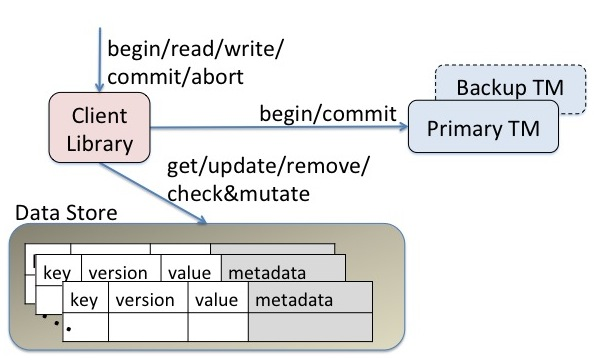
\includegraphics[width=0.40\textwidth]{FragolaComponents.jpg}
}
\caption{\small Transaction processing architecture: A client library exposes an  API for  executing transactions of data store operations. 
A centralized Transaction Manager (TM) handles transaction begin and commit requests, while data is written directly to the 
underlying data store. The TM has a backup for high availability.}
\label{fig:components}
\end{figure}

Figure~\ref{fig:components} depicts, at a high level, the primary components of the TPS architecture,  
their APIs, and interaction with the data store. 
In many TPSs, transaction processing follows the following general schema, 
outlined in Algorithm~\ref{alg:schema}, while systems vary in their implementations of each of the steps.

\remove{
For example, whereas most systems rely on a centralized service for timestamp allocation~\cite{OmidICDE2014,Omid2017,tephra,Percolator2010}, this is not essential~\cite{cockroach}; similarly, validation (conflict detection) can use a centralized service~\cite{OmidICDE2014,Omid2017,tephra}, per-transaction entries in a global table~\cite{cockroach}, or distributed locking and validation~\cite{Percolator2010}. 
Different ways to implement this schema are  discussed in Section~\ref{sec:context}.
We now overview the phases a transaction goes through, focusing on Omid's approach.
}

\begin{algorithm}[tb]
\begin{algorithmic}[1]
\small
\Procedure{begin}{}
\State obtain read timestamp $ts_r$ 
\EndProcedure
%\Statex

\Procedure{write}{$ts_r$, key, \inred{fields, values}} 
\\ \Comment transactional write
\State optionally check for conflicts and abort if found 
\State indicate write intent for key with \inred{values} and $ts_r$
\State add key to local write-set
\EndProcedure
%\Statex

\Procedure{read}{$ts_r$, key} \Comment transactional read
\If{key has write intent}
	\State resolve, possibly abort writing transaction \label{l:resolve}
\EndIf
\State return highest version   $\le ts_r$ of key
\EndProcedure

%\Statex

\Procedure{commit}{$ts_r$, write-set}
\Statex \Comment check for write-write conflicts  \label{l:validate}
\State obtain commit timestamp $ts_c$
\If{validate(write-set, $ts_r$)}  
%	\Statex \Comment commit all write intents with version $ts_c$
	\State write commit  version $ts_c$ to persistent commit entry \label{l:commit}
\Else
	\State abort	
\EndIf
\State post-commit: update meta-data
\EndProcedure

\end{algorithmic}
\caption{TPS operation schema.} 
\label{alg:schema}

\end{algorithm} 

Many systems employ a centralized \emph{transaction manager (TM)\/} service~\cite{Percolator2010,OmidICDE2014,Omid2017,tephra},
for timestamp allocation and other functionalities. 
 Because a centralized service can become a single point of failure, the TM is sometimes implemented
 as a primary-backup server pair to ensure its continued availability following failures.

\mypara{Begin.} 
  When a transaction begins, it obtains a read timestamp (version) $ts_r$ for reading its consistent snapshot.
  %, and unique transaction id.   The two can be combined (i.e., $ts_r$ can serve as the  transaction id, provided that it is unique).
 % In most cases, this is done using the centralized TM~\cite{Percolator2010,OmidICDE2014,Omid2017,tephra}. 
%  In CockroachDB, the timestamp is based on a local clock that is ``close to'' real-time and preserves causality 
 % across regions, and unique transaction ids are used to break ties in case timestamps (from different regions) are identical. 

\mypara{Transactional writes.} 
 During a transaction, a write operation indicates its \emph{intent} to write to a single object a certain new value with a certain version number.
%a dedicated \emph{commit} column in the object indicates that the write is tentative.
In Omid, the version is the transaction's $ts_r$, which exceeds all versions written by transactions that committed before it  began. 
%Note that the version order among concurrent transactions that  attempt to update the same key is immaterial, 
%since all but one of these transactions are doomed to abort. 
% It is possible to buffer write intents locally (at the client) in the course of the transaction, and add the write intents to the data store at commit time~\cite{Percolator2010}.
% In some solutions writes check for conflicts before declaring their intents~\cite{cockroach}, whereas in others, 
% all conflict detection is deferred to commit time~\cite{Percolator2010,OmidICDE2014,Omid2017,tephra}. 

\mypara{Transactional reads.} 
The reads of a given transaction obtain a consistent snapshot of the data store at logical time (i.e., version) $ts_r$.
Each read operation retrieves the value of a single object associated with the highest timestamp that is 
smaller or equal to the transaction's $ts_r$. 

On encountering a write intent, read cannot proceed without determining whether the tentative write should be included in its snapshot,
for which it must know the writing transaction's commit status. 
To this end, TPSs keep per-transaction \emph{commit entries}, which are the source of truth regarding the transaction status 
(pending, committed, or aborted). 
This entry is updated in line~\ref{l:commit} of Algorithm~\ref{alg:schema} 
and is checked in order to resolve write intents in line~\ref{l:resolve}.
%In some cases~\cite{Percolator2010,cockroach}, when the status of the writing transaction  is undetermined, the read forcefully aborts
%it by updating the commit entry accordingly, as explained below.

%Similarly, the solution we implement in \sys\ forces the transaction with the pending write intent to abort. 

  \mypara{Commit.} 
  Commit occurs in four steps: \vspace{-0.3cm}
  \begin{enumerate}
    \setlength{\itemsep}{0pt}
    \setlength{\parskip}{0pt}
    \setlength{\parsep}{2pt}  
  \item
  Obtain a commit timestamp, $ts_c$. 
%  In most cases, e.g.,~\cite{Percolator2010,OmidICDE2014,Omid2017,tephra}, 
 % this is the value of some global clock maintained by a centralized entity. 
  \item \emph{Validate} that the transaction does not conflict with any concurrent transaction that has committed since it 
had begun.  For SI, checks for write-write conflicts only. 
%If write intent indications are buffered, they are added at this point~\cite{Percolator2010}.
%Validation can be centralized~\cite{OmidICDE2014,Omid2017,tephra} or distributed~\cite{Percolator2010,cockroach}. 


\item \emph{Commit} or abort in one  irrevocable atomic step by persistently writing to the \emph{commit entry}. 
%  which can reside in a global table~\cite{Omid2017,cockroach} or alongside the first  key written by 
 % the transaction~\cite{Percolator2010}.  
  
 \item \emph{Post-commit}: 
  Finally, a transaction changes its write intents to
  persistent writes in case of commit, and removes them in case of abort. This
  step is not essential for correctness, but reduces the overhead of future transactions. It
  occurs after the transaction is persistently committed or aborted via the commit entry, 
  and can be done asynchronously.
  %in
  %order to reduce the overhead of future transactions (by sparing them the need to check the commit entry)
  %and to garbage collect   obsolete information. 
 \end{enumerate}
 
  \remove{Note that whenever a transaction encounters a write
  indication in the collect phase it must access the commit entry in order to
  check the transaction's commit status. Once the post-commit phase is over, future
  transactions no longer incur this overhead for keys updated by the terminated
  transaction.}

\subsection{Big data platforms}
\label{ssec:bigdata}

{\inred{

Apache HBase is one of the most scalable key-value storage technologies available today. 
Phoenix complements the HBase storage tier with a query processing (compute)
tier. The latter scales independently (the current scalability goal is $10{,}000$ query servers). 
Phoenix compiles every SQL statement into a plan, and executes it on one or more servers. 
Its query processing code invokes the underlying HBase for low-level data access, and a 
TPS (Omid or Tephra) for transaction management, through client libraries. 

Wherever possible, Phoenix strives to push computation close to data (e.g., for filtering
and aggregation), in order to minimize cross-tier communication. For this, it makes 
extensive use of server-side stored procedures, which in HBase are supported by the 
non-intrusive {\em coprocessor\/} mechanism. Omid uses HBase coprocessors too, both for 
performance improvements and for specific services, such as garbage collection of redundant 
data. 
}}